O transporte de um escalar segundo uma função parabólica
e submetido a um escoamento monofásico de um fluido
newtoniano e incompressível com elevado número de \textit{Reynold} ($\textit{Re} \rightarrow \infty$)
é conhecido como um \textit{Escoamento Puramente Convectivo}.
Neste tipo de escoamento, espera-se que não ocorra difusão do escalar.
Para os métodos de aproximação como \textit{MEF} e \textit{MDF},
é possível observar a presença de oscilações espúrias. 
Como mencionado anteriormente, diversos esquemas podem ser utilizados para reduzir essas
oscilações. Apresentaremos nesta seção a utilização do esquema de
\textit{Taylor-Galerkin} na redução das oscilações espúrias em comparação ao esquema \textit{Galerkin}.
A \ref{conveccao} apresenta esquematicamente o problema e
a dinâmica do transporte do escalar.

\vspace{0.5cm}
\begin{figure}[H]
\begin{center}
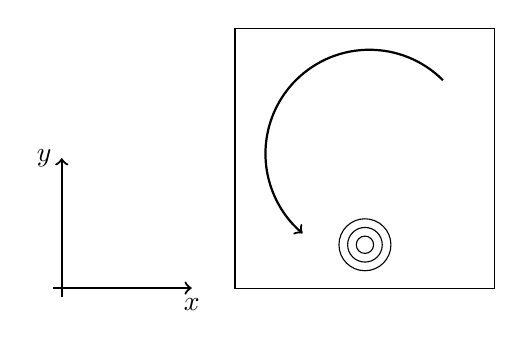
\begin{tikzpicture}[scale=1.1]
 \draw (0,0) -- (3,0) -- (3,3) -- (0,3) -- cycle;

 \draw [->,thick] (2.4,2.4) arc (45:230:1.2);
 
 \draw [->,thick] (-2,-0.1)--(-2,1.5) node[left] {$y$};
 \draw [->,thick] (-2.1,0)--(-0.5,0) node[below] {$x$};

 \draw (1.5,0.5) circle (0.3);
 \draw (1.5,0.5) circle (0.2);
 \draw (1.5,0.5) circle (0.1);

\end{tikzpicture}
\end{center}
\caption{Transporte de um escalar num Escoamento Puramente Convectivo}
\label{conveccao}
\end{figure}

\medskip
O domínio foi discretizado utilizando uma malha 
triangular linear com 1231 nós e 2340 elementos. 
A equação que governa o escoamento puramente convectivo
de um escalar qualquer $c$ é definida como:

\begin{equation}
 \frac{\partial c}{\partial t} 
 + 
 \textbf{v} \cdot \nabla c
 = 0
\end{equation}

\noindent
onde $\textbf{v} = (u,v)$ é o vetor velocidade e suas componentes 
são definidas como: $u = -y$ e $v = x$. Portanto, espera-se que
dado um campo escalar inicial, o mesmo seja deslocado pelo campo
de velocidade sem que ocorra difusão, isto é, seu perfil não deve
ser alterado enquanto o escoamento acontece. Qualquer alteração
no perfil do campo escalar é considerado como erro numérico.

\medskip
\noindent
As condições de contorno e inicial utilizadas foram:

\begin{itemize}
     \item \textit{condição de contorno}: o campo escalar $c$ é especificado
      com o valor $c=0$ no contorno da geometria.

     \item \textit{condição inicial}: o campo escalar é definido segundo
      a função parabólica $c = 1 - x^2 - y^2$.
\end{itemize}

\medskip
A \ref{perfil c} apresenta a comparação do perfil do campo escalar $c$ para os esquemas Galerkin e
Taylor-Galerkin em diferentes posições no eixo de rotação conforme o escoamente ocorre. É possível observar que em ambos
os esquemas é apresentado oscilações espúrias. No esquema Taylor-Galerkin, porém, tais
oscilações são amortecidas diferentemente do esquema Galerkin onde podemos observar que
as oscilações espúrias aumentam e o perfil do campo escalar torna-se completamente distorcido. 

\begin{center}
\begin{figure}[H]
     \centering
     \begin{minipage}{.5\linewidth}
      \centering
      \includegraphics[scale=0.53]{./02_chaps/cap_validation/figure/convection_0.pdf}\\
      (a)
     \end{minipage}%
     \begin{minipage}{.5\linewidth}
      \centering
      \includegraphics[scale=0.53]{./02_chaps/cap_validation/figure/convection_300.pdf}\\
      (b)
     \end{minipage}
     \begin{minipage}{.5\linewidth}
      \centering
      \includegraphics[scale=0.53]{./02_chaps/cap_validation/figure/convection_600.pdf}\\
      (c)
     \end{minipage}%
     \begin{minipage}{.5\linewidth}
      \centering
      \includegraphics[scale=0.53]{./02_chaps/cap_validation/figure/convection_950.pdf}\\
      (d)
     \end{minipage}
     \medskip
     \caption{Comparação do perfil de $c$ para os esquemas Galerkin e Taylor-Galerkin em diferentes posições do eixo de rotação:
     (a) ponto inicial, 
     (b) 1/4 da rotação,
     (c) 1/2 da rotação e
     (d) 3/4 da rotação.}
     \label{perfil c}
\end{figure}
\end{center}

\vspace{-1cm}
As \ref{galerkin} e \ref{taylor} apresentam a disposição espacial das oscilações espúrias
para os esquemas Galerkin e Taylor-Galerkin respectivamente. Como mencionado anteriormente,
as oscilações apresentadas no esquema Galerkin distorcem completamente o campo escalar $c$
enquanto no esquema Taylor-Galerkin as mesmas são amortecidas como esperado. Portanto,
para os problemas onde as oscilações espúrias estão presentes,
o esquema Taylor-Galerkin é superior ao esquema Galerkin.

\vspace{0.5cm}
\begin{figure}[H]
     \centering
     \begin{minipage}{.5\linewidth}
      \centering
      \includegraphics[scale=0.2]{./02_chaps/cap_validation/figure/galerkin_0.png}\\
      (a)
     \end{minipage}%
     \begin{minipage}{.5\linewidth}
      \centering
      \includegraphics[scale=0.2]{./02_chaps/cap_validation/figure/galerkin_300.png}\\
      (b)
     \end{minipage}
     \begin{minipage}{.5\linewidth}
      \centering
      \includegraphics[scale=0.2]{./02_chaps/cap_validation/figure/galerkin_600.png}\\
      (c)
     \end{minipage}%
     \begin{minipage}{.5\linewidth}
      \centering
      \includegraphics[scale=0.21]{./02_chaps/cap_validation/figure/galerkin_950.png}\\
      (d)
     \end{minipage}
     \medskip
     \caption{Oscilações espúrias para o esquema Galerkin em diferentes posições do eixo de rotação:
     (a) ponto inicial, 
     (b) 1/4 da rotação,
     (c) 1/2 da rotação e
     (d) 3/4 da rotação.}
     \label{galerkin}
\end{figure}

\begin{figure}[H]
     \centering
     \begin{minipage}{.5\linewidth}
      \centering
      \includegraphics[scale=0.2]{./02_chaps/cap_validation/figure/taylor_0.png}\\
      (a)
     \end{minipage}%
     \begin{minipage}{.5\linewidth}
      \centering
      \includegraphics[scale=0.2]{./02_chaps/cap_validation/figure/taylor_300.png}\\
      (b)
     \end{minipage}
     \begin{minipage}{.5\linewidth}
      \centering
      \includegraphics[scale=0.2]{./02_chaps/cap_validation/figure/taylor_600.png}\\
      (c)
     \end{minipage}%
     \begin{minipage}{.5\linewidth}
      \centering
      \includegraphics[scale=0.2]{./02_chaps/cap_validation/figure/taylor_950.png}\\
      (d)
     \end{minipage}
     \medskip
     \caption{Oscilações espúrias para o esquema Taylor-Galerkin em diferentes posições do eixo de rotação:
     (a) ponto inicial, 
     (b) 1/4 da rotação,
     (c) 1/2 da rotação e
     (d) 3/4 da rotação.}
     \label{taylor}
\end{figure}

